%% The following is a directive for TeXShop to indicate the main file
%%!TEX root = diss.tex

\chapter{Conclusions}
\label{chap:conclusion}

This dissertation has examined the influence of attention and linguistic salience on perceptual learning in speech perception.
Through explicit instructions and experimental manipulations, listeners were induced towards a more comprehension-oriented attentional set or a more perception-oriented attentional set.
Those participants in conditions biased towards comprehension showed larger perceptual learning effects than those in conditions biased more towards perception.
I adopted a predictive coding framework \citep{Clark2013} that provides an intuitive model of perceptual learning and has been computationally implemented \citep{Kleinschmidt2011}.
However, the attentional mechanism in the predictive coding framework does not work well for some instances of visual attention \citep{Block2013}, or for the current results.
I propose a new attentional mechanism for predictive coding, one in which attention blocks error propagation beyond the level to which attention is directed.  Such a mechanism explains both the previous findings and the current results.

\begin{figure*}[!ht]
\caption{Distribution of cross over points for each participant across comparable exposure tokens in all experiments.}
\label{fig:exp123xoverdist}
\begin{center}
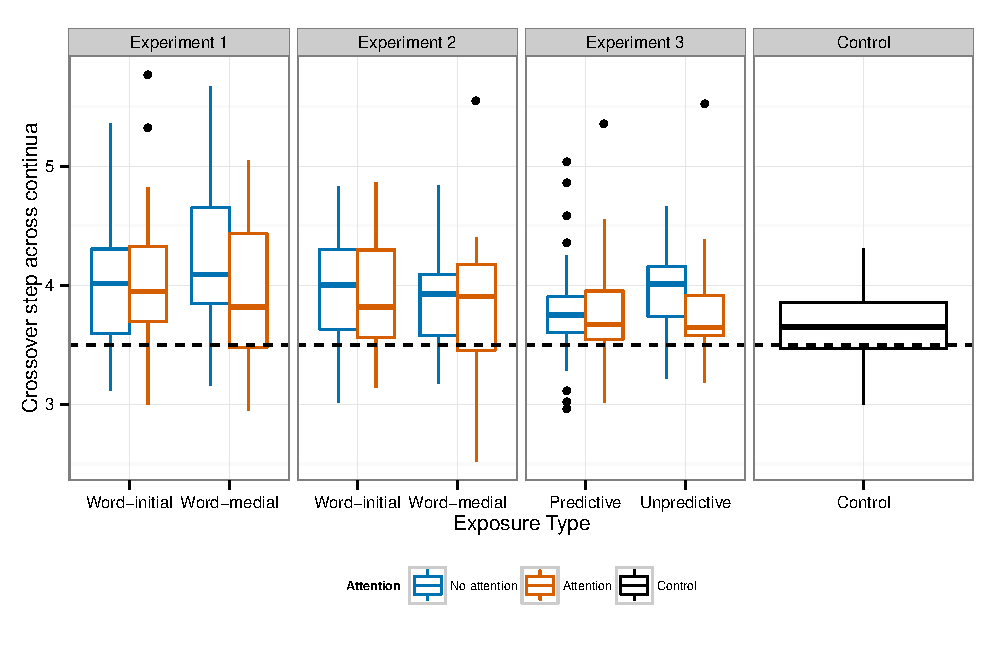
\includegraphics[width=\textwidth]{graphs/exp123_xoverdist}
\end{center}
\end{figure*}


\section{Attentional control of perceptual learning}

The findings of Experiment 1 suggest also that perceptual learning is not a wholly automatic process.  
Although all participants showed perceptual learning effects, those exposed to the ambiguous sound with increased lexical bias only showed larger perceptual learning effects when the instructions about the speaker's ambiguous sound were withheld.  
Attention on the ambiguous sound equalized the perceptual learning effects across lexical bias.
However, in Experiment 2, there is no such effect of attention, suggesting that the ambiguous sounds that were farther away from the canonical production drew the listener's attention to those sounds.

One question raised by the current results is whether attention always decreases perceptual learning.  
The instructions used to focus the listener's attentional set framed the ambiguity in a negative way, with listeners being cautioned to listen carefully to ensure they made the correct decision.  
If the attention were directed to the ambiguous sound by framing the ambiguity in a positive way, would we still see the same pattern of results?
The current mechanism would predict that attention of any kind to signal properties would block the propagation of errors, reducing perceptual learning.
This prediction will be tested in future work.

\section{Specificity versus generalization in perceptual learning}

The results of this dissertation speak to dichotomy between specificity and generalization found in perceptual learning work. 
In Experiment 1, greater perceptual learning was shown by participants exposed to ambiguous sounds later in the words, not to those at the beginnings of words. 
And yet, the testing continua consisted of stimuli with the sibilant at the beginnings of words, which are more similar to the words beginning with the ambiguous sound.

The effect of attention in Experiments 1 and 2 suggest that when speakers are focused on the signal, or have their attention drawn to the signal, they are less likely to generalize across forms.
When attention on the signal is not present, errors can propagate more widely causing greater updating.
These different modes of perceptual learning may account for some differences that have been observed in the literature.
While visually-guided perceptual learning shows comparable effects to lexically-guided perceptual learning \citep{vanLinden2007}, lexically-guided perceptual learning is more likely to be expanded to new contexts \citep{Norris2003, Kraljic2008a}, though with some restrictions \citep{Mitterer2013}, than visually-guided perceptual learning \citep{Reinisch2014}.
%The methodologies used to induces perceptual learning in these two ways differ in ways that might confound this generalization.
%Lexically-guided perceptual learning uses relatively few ambiguous tokens, but ones embedded in an array of lexical contexts whereas visually-guided perceptual learning uses many more ambiguous token instances, but embedded in very few frames.

\section{Effect of increased linguistic expectations}

Comprehension-oriented attentional sets were promoted mainly through the task demands and the use of increased lexical and semantic expectations.
The conditions that correspond most closely to those in other lexically-guided perceptual learning experiments \citep{Norris2003, Kraljic2005} are those participants not told of the ambiguous sound in Experiment 1.
Under those conditions, there is a clear effect of lexical bias, such that listeners exposed to ambiguous stimuli with greater lexical bias update their speaker-specific category for that sound more.

\section{Category atypicality}

In Experiment 2, there was no effect of attention or lexical bias on perceptual learning, with a stable effect present for all listeners.
There are two potential, non-exclusive explanations for the lack of effects.
As stated above, the increased distance to the canonical production drew the listener's attention to the ambiguous productions, resulting in a perception-oriented attentional set.
The second potential explanation is that the productions farther from canonical produce a weaker effect on the updating of a listener's categories, as predicted from the neo-generative model in \citep{Pierrehumbert2002}.
This explanation is supported in part by the weaker correlation between word endorsement rate and crossover point found in Experiment 2, and the findings of \citet{Sumner2011} where the most perceptual learning was found when the categories begin like the listener expects and gradually shift toward the speaker's actual boundaries over the course of exposure.
This explanation could be tested straightforwardly by implementing the same gradual shift paradigm used in \citet{Sumner2011} with the manipulations used in this dissertation.

An interesting extension to the current findings would be to observe the perceptual learning effects in a cognitive load paradigm.  Speech perception under cognitive load has shown to have greater reliance on lexical information due to weaker initial encoding of the signal \citep{Mattys2011}.  Following exposure to a modified ambiguous category, we might expect to see less perceptual learning if the exposure was accompanied by high cognitive load.  However, \citet{Scharenborg2014} found that hearing loss of older participants did not significantly influence their perceptual learning.  Therefore it may be that perceptual learning would likewise be similar across cognitive loads.
Higher cognitive loads, however, might allow for more atypical ambiguous stimuli to be learned, due to the increased reliance on lexical information during initial encoding.

\section{Conclusion}

This dissertation investigated the influences of attention and linguistic salience on perceptual learning in speech perception.
Perceptual learning was modulated by the attentional set of the listener.
Decreased linguistic salience by increasing linguistic expectations induced more comprehension-oriented attentional sets, resulting in larger perceptual learning effects.
Inducing perception-oriented attentional sets through explicit instructions or making the modified sound category more atypical resulted in smaller perceptual learning effects.
These results support a greater role of attention than previously assumed in predictive coding frameworks, such as the proposed propagation-blocking mechanism.
Finally, these results suggest that the degree to which listeners perceptually adapt to a new speaker is under their control to a degree, but given the robust perceptual learning effects across all conditions, perceptual learning is a largely automatic process.


